\documentclass[twocolumn,aps]{revtex4-1}

% allows special characters (including æøå)
\usepackage[utf8]{inputenc}
%\usepackage [norsk]{babel} %if you write norwegian
\usepackage[english]{babel}  %if you write english
\usepackage{tikz}             % Added for drawing the FFNN figure 
\usetikzlibrary{arrows.meta,decorations.pathreplacing}

\usepackage{physics,amssymb}  % mathematical symbols (physics imports amsmath)
\usepackage{graphicx}         % include graphics such as plots
%\usepackage[table]{xcolor}
%\usepackage{xcolor}           % set colors
\usepackage{hyperref}         % automagic cross-referencing 
\usepackage{float}			  % force placement of tables and figures
\usepackage{comment}
%\usepackage[authoryear]{natbib}
\usepackage{algorithm}
\usepackage{amsthm}
\usepackage{algpseudocode}
\usepackage{multirow}
\usepackage{enumerate}




\newtheorem{prop}{Proposition}[section]

\begin{document}

\title{Implementation of a Feed Forward Neural Network, studied on Sparse Regression and MNIST Classification}
\date{\today}               
\author{
    Anton Nicolay Torgersen 
}
\affiliation{University of Oslo}


\newpage


%Abstract: accurate and informative? Total number of possible points: 5

    \begin{abstract}
Spotting waste is important abstract.  Methods and REsults.
\end{abstract}


    \maketitle
    \thispagestyle{empty} % Removes page number from the title page

    


% Introduction: status of problem and the major objectives. Total number of possible points: 10


\section{Introduction}
Machine learning has found widespread use in reason years in diverse fields of study where traditional methods struggle to find patterns in complex data.
Especially in the image recognition task has it become a standard tool.
WE will do this on the waste dataset to try and detect where a waste should be placed.

MORE INTRODUCTION


\section{Methods}\label{section:methods}
This section details the theory and methodology used to implement a flexible feed-forward neural network (FFNN) from scratch. 
We will first describe the data preparation process for the regression and classification tasks. 
Following this, we detail the fundamental building blocks of the FFNN, including its architecture, the activation functions (Sigmoid, ReLU, Leaky ReLU), the cost functions (Mean Squared Error and Cross-Entropy), and the gradient-based optimization algorithms (RMSprop, ADAM). 
Finally, we will discuss the implementation details and code structure.

\subsection{Data Preparation}
Location of the dataset.
How it is structured.
Resizing images to smaller sizes using numpy, but with consistent down scaling interms of whole numbers.
How we standardized the data and split it into training and test sets.
Usage og RGB and greyscale images.

\begin{figure*}[t]
    \centering
    \includegraphics[width=\linewidth]{Figures/ExampleImages.png}
    \caption{Four examples of images in the data set}
    \label{fig:Training_struggle}
\end{figure*}




\subsubsection{generating more data}
Transforming the data with rotations, flips, crops etc to generate more data for training the NN.

How it looks and the data augmentations

\begin{figure*}[t]
    \centering
    \includegraphics[width=\linewidth]{Figures/ExampleAugmentation.png}
    \caption{How each Image in the training set was augmented to increase training size}
    \label{fig:Training_struggle}
\end{figure*}



\subsection{Logistic Regression}

\subsection{FFNN Method}
A feed-forward neural network (FFNN) is a model that approximates a function by composing multiple simpler functions. 
The network is organized into layers: an input layer, one or more hidden layers, and an output layer, as shown in Fig. \ref{fig:ffnn-arch}.

\begin{figure}[htbp] % No asterisk, so it stays in one column
    \centering
    % This scales the entire drawing to fit the column width
    \resizebox{\columnwidth}{!}{ 
    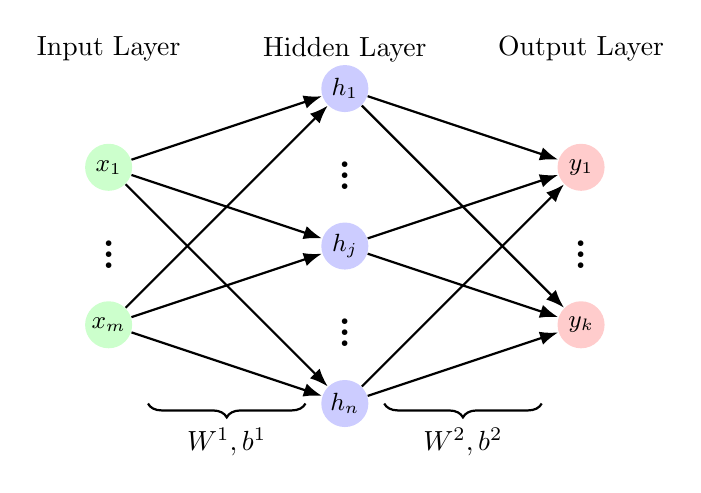
\begin{tikzpicture}[
        node distance=2cm, 
        neuron/.style={circle, fill=blue!20, minimum size=17pt, inner sep=0pt, font=\small},
        input/.style={neuron, fill=green!20},
        output/.style={neuron, fill=red!20},
        arrow/.style={-Latex, thick},
        dots/.style={font=\Huge, minimum height=1cm, inner sep=0, outer sep=0, node distance=0.5cm}
    ]
        % Input Layer
        \node[input] (I1) at (0, 2) {$x_1$};
        \node[input] (I2) at (0, 0) {$x_m$};
        \node[dots] (Idots) at (0, 1) {$\vdots$};

        % Hidden Layer
        \node[neuron] (H1) at (3, 3) {$h_1$};
        \node[neuron] (H2) at (3, 1) {$h_j$};
        \node[neuron] (H3) at (3, -1) {$h_n$};
        \node[dots] (Hdots) at (3, 2.0) {$\vdots$};
        \node[dots] (Hdots2) at (3, 0.0) {$\vdots$};

        % Output Layer
        \node[output] (O1) at (6, 2) {$y_1$};
        \node[output] (O2) at (6, 0.0) {$y_k$};
        \node[dots] (Odots) at (6, 1) {$\vdots$};

        % Arrows
        \draw[arrow] (I1) -- (H1); \draw[arrow] (I1) -- (H2); \draw[arrow] (I1) -- (H3);
        \draw[arrow] (I2) -- (H1); \draw[arrow] (I2) -- (H2); \draw[arrow] (I2) -- (H3);
        \draw[arrow] (H1) -- (O1); \draw[arrow] (H1) -- (O2);
        \draw[arrow] (H2) -- (O1); \draw[arrow] (H2) -- (O2);
        \draw[arrow] (H3) -- (O1); \draw[arrow] (H3) -- (O2);
        
        % Layer Labels
        \node at (0, 3.5) {Input Layer};
        \node at (3, 3.5) {Hidden Layer};
        \node at (6, 3.5) {Output Layer};
        
        % Braces
        \draw [decorate, decoration={brace, amplitude=5pt, mirror}, thick] (0.5, -1) -- (2.5, -1) node [midway, below=5pt] {$W^1, b^1$};
        \draw [decorate, decoration={brace, amplitude=5pt, mirror}, thick] (3.5, -1) -- (5.5, -1) node [midway, below=5pt] {$W^2, b^2$};

    \end{tikzpicture}
    } % End of \resizebox
    \caption{A simple Feed Forward Neural Network (FFNN) architecture with one input layer, one hidden layer, and one output layer. 
    Each neuron in a layer is connected to every neuron in the subsequent layer through weights ($W$) and biases ($b$).}
    \label{fig:ffnn-arch}
\end{figure}

\subsubsection{Prediction}

The process begins with the \textit{feed-forward pass}. For a given input vector $\boldsymbol{x}$, the activation $\boldsymbol{a}^l$ of layer $l$ is computed based on the activation of the previous layer $\boldsymbol{a}^{l-1}$ (where $\boldsymbol{a}^0 = \boldsymbol{x}$):

$$
\boldsymbol{z}^l = \boldsymbol{W}^l \boldsymbol{a}^{l-1} + \boldsymbol{b}^l
$$
$$
\boldsymbol{a}^l = f_l(\boldsymbol{z}^l)
$$
where $\boldsymbol{W}^l$ and $\boldsymbol{b}^l$ are the weight matrix and bias vector for layer $l$, and $f_l$ is the activation function. 
This process is repeated until the final output $\boldsymbol{a}^L = \hat{\boldsymbol{y}}$ is computed.

\subsubsection{Learning}

The network "learns" by minimizing a \textit{cost function} $\mathcal{C}(\boldsymbol{W}, \boldsymbol{b})$, which measures the discrepancy between the predicted output $\hat{\boldsymbol{y}}$ and the true target $\boldsymbol{y}$. 
This minimization is achieved using gradient-based optimization.

The \textit{backpropagation} algorithm is used to efficiently compute the gradient of the cost function with respect to every weight and bias in the network. 
It is an application of the chain rule, starting from the output layer and moving backward, here for a single training example:
\begin{enumerate}
    \item Compute the error $\boldsymbol{\delta}^L$ at the output layer $L$:
    $$ \boldsymbol{\delta}^L = \nabla_{\boldsymbol{a}^L} \mathcal{C} \odot f_L'(\boldsymbol{z}^L) $$
    \item Propagate the error backward to compute the error $\boldsymbol{\delta}^l$ for layer $l$:
    $$ \boldsymbol{\delta}^l = ((\boldsymbol{W}^{l+1})^T \boldsymbol{\delta}^{l+1}) \odot f_l'(\boldsymbol{z}^l) $$
    \item The gradient of the cost function with respect to the parameters of layer $l$ is then:
    $$ \nabla_{\boldsymbol{W}^l} \mathcal{C} = \boldsymbol{\delta}^l (\boldsymbol{a}^{l-1})^T $$
    $$ \nabla_{\boldsymbol{b}^l} \mathcal{C} = \boldsymbol{\delta}^l $$
\end{enumerate}
These gradients are then used by an optimization algorithm to update the weights and biases.



\subsubsection{Hyperparameters}
Just as with project 1, there are several hyperparameters to tune when setting up the FFNN, to get the best results.

\begin{itemize}
    \item \textbf{Learning Rate ($\eta$):} Controls how much to change the model in response to the estimated error each time the model weights are updated.
    \item \textbf{Number of Epochs:} The number of times the learning algorithm will work through the entire training dataset.
    \item \textbf{Batch Size:} The number of training examples utilized in one learning iteration.
    \item \textbf{Number of Hidden Layers and Units:} The architecture of the network, including how many hidden layers to use and how many neurons in each layer.
    \item \textbf{Activation Functions:} The choice of activation functions for each layer (e.g., ReLU, sigmoid, tanh).
\end{itemize}
In the results we will go through them to find a good approximation of the optimal parameters.
It is believed that deeper networks with more layers can capture more complex patterns, but they are also harder to train.

For more on FFNNs see chapter 1 and 2 in \cite[Nielsen]{NeuralNetworks}.


\subsection{Different Building Blocks}

\subsubsection{Cost Functions}

\textbf{Mean Squared Error (MSE)}
For regression tasks, we use the Mean Squared Error (MSE) cost function, which is identical to the one used in \cite{project1}. 
For a set of $n$ samples, it is:
$$
\mathcal{C}_{MSE}(\boldsymbol{W}, \boldsymbol{b}) = \frac{1}{n} \sum_{i=1}^n (y_i - \hat{y}_i)^2
$$
Its derivative with respect to a single final activation $\hat{y}_i$ (which is $a^L_i$) is computed as:
$$
\frac{\partial \mathcal{C}_i}{\partial \hat{y}_i} = 2(\hat{y}_i - y_i)
$$
where $\mathcal{C}_i = (y_i - \hat{y}_i)^2$ is the per-sample cost.

We extend this cost function to include $L_1$ and $L_2$ regularization, which helps prevent overfitting by penalizing large weights. 
The parameter $\lambda$ controls the strength of the regularization, see 3.4 \cite{hastie}.
\\

\textbf{L1 Regularization (LASSO):} 
The $L_1$ norm adds a penalty proportional to the absolute value of the weights, which encourages sparsity. This is the same technique used in LASSO regression in \cite{project1}. The cost function becomes:
$$
\mathcal{C}_{L1} = \mathcal{C}_{MSE} + \frac{\lambda}{2n} \sum_{l=1}^L \sum_{ij} |W^l_{ij}|
$$
The gradient of this term is:
$$
\nabla_{\boldsymbol{W}^l} \mathcal{C}_{L1} = \nabla_{\boldsymbol{W}^l} \mathcal{C}_{MSE} + \frac{\lambda}{2n} \cdot \text{sign}(\boldsymbol{W}^l)
$$

Where handling the non-differentiable L1 norm requires using a sub-gradient. For optimization, we use the sub-gradient of the penalty term, which is $\frac{\lambda}{2n} \cdot sign(W^{l})$, see 3.4.4 \cite{hastie}.
\\

\textbf{L2 Regularization (Ridge):} 
The $L_2$ norm adds a penalty proportional to the square of the weights. This is the same regularization technique used in Ridge regression in \cite{project1}. The cost function becomes:
$$
\mathcal{C}_{L2} = \mathcal{C}_{MSE} + \frac{\lambda}{2n} \sum_{l=1}^L \sum_{ij} (W^l_{ij})^2
$$
The gradient of this term, added during backpropagation, is:
$$
\nabla_{\boldsymbol{W}^l} \mathcal{C}_{L2} = \nabla_{\boldsymbol{W}^l} \mathcal{C}_{MSE} + \frac{\lambda}{n} \boldsymbol{W}^l
$$


\subsubsection{Activation Functions}
Disregarding the linear activation function used in the output layer for regression, we have three commonly used activation functions for the hidden layers of the network.
These are non-linear so that the FFNN model doesn't become the same as a network with zero hidden layers. 
i.e. matrices multiplied together is still a matrix.
\\

\textbf{Sigmoid}
An exponential function that has a range from 0 to 1, and a continues derivative.
A common problem with this method is diminishing gradients where the network will struggle to learn for large gradients. 
$$
\sigma(z) = \frac{1}{1+e^{-z}}
$$



\textbf{ReLU}
The Rectified Linear Unit (ReLU) is a piecewise linear function that outputs the input directly if it is positive; otherwise, it will output zero. This function has become the default activation function for many types of neural networks because a model that uses it can often converge faster than those using sigmoid or tanh functions.
$$
\text{ReLU}(z) = \max(0, z)
$$
\\

\textbf{Leaky ReLU}
The Leaky ReLU is a variant of the ReLU that allows a small, non-zero gradient $\alpha$ when the input is negative. 
This helps to mitigate the dying ReLU problem, where neurons can become inactive and stop learning entirely.
$$
\text{Leaky ReLU}(z) = \max(\alpha z, z)
$$

For more on activation functions see 14.12 in the lecture notes \cite{compfys}.

\subsubsection{Optimization Algorithms}
In a previous paper \cite{project1}, we implement three different gradient-based optimization algorithms to update the weights and biases of the gradient descent.
Where the most important where Stochastic Gradient Descent (SGD), RMSprop and Adam.
These methods are widely used in training neural networks due to their efficiency and effectiveness in handling large datasets (SGD) and adapting learning rates (RMSprop and Adam).
\\

\textbf{Stochastic Gradient Descent (SGD)} is an optimization method that approximates the full batch gradient by utilizing a small, randomly sampled subset of the data, known as a mini-batch $B_t$ of size $m$, at each iteration. 
This introduces stochastic noise into the optimization path. 
The update rule for SGD is the same as for standard gradient descent, but the gradient is computed over the mini-batch.
See 8.3.1 in \cite{Goodfellow} for more details.
\\

\textbf{RMSprop} is an optimization method designed to address the aggressively diminishing learning rates found in other adaptive methods like AdaGrad. 
It approximates a running average of the squared gradients by utilizing an exponentially decaying moving average, $E_t$, at each iteration. 
This helps prevent the learning rate from diminishing too quickly. 
The update rule for RMSprop scales the gradient by the inverse of this moving average: 
\begin{align*} 
    \theta_{t+1} &= \theta_t - \frac{\eta}{\sqrt{E_t + \epsilon}} \odot \nabla_{\theta} J(\theta_t) 
\end{align*} 
where $E_t$ is the moving average of the squared gradients and $\epsilon$ is a small smoothing constant. 
See 8.5.2 in \cite{Goodfellow}.
\\

\textbf{Adam} (Adaptive Moment Estimation) is an optimization method that combines the momentum method with the adaptive learning rate scaling of RMSprop. 
It maintains two exponentially decaying moving averages: a moving average of the gradients ($m_t$, the first moment) and a moving average of the squared gradients ($v_t$, the second moment). 
Adam is often considered a highly efficient and stable general-purpose optimizer. 
The update rules are:

\begin{align*} 
    m_{t+1} &= \beta_1 m_t + (1 - \beta_1) \nabla_{\theta} J(\theta_t) \\ 
    v_{t+1} &= \beta_2 v_t + (1 - \beta_2) (\nabla_{\theta} J(\theta_t))^2 \\ 
    \theta_{t+1} &= \theta_t - \frac{\eta}{\sqrt{v_{t+1} + \epsilon}} \odot m_{t+1} 
\end{align*} 
where $\beta_1$ and $\beta_2$ are decay rates for the moments and $\epsilon$ is a small smoothing constant. 
See 8.5.3 in \cite{Goodfellow}.
\\

The implementation of these methods for the FFNN followed a straightforward approach using the update rules or restrictions above. 
See the GitHub repository \cite{rep2} for the exact implementation.

\subsection{Image Classification}

When applying our FFNN model to an image classification task, one only needs to make a few adjustments to the architecture and cost function to suit the nature of classification problems.
Which we will then demonstrate on the MNIST dataset of handwritten digits.
This alternations to the architecture follow the book shown in \cite{NeuralNetworks} chapter 3.
\\

\subsubsection{Output layer}
For multiclass classification tasks, the output layer of the FFNN is modified to use the softmax activation function.
The softmax function converts the raw output scores (logits) from the final layer into probabilities for each class.
Given an input vector $\boldsymbol{z}$ from the final layer, the softmax function is defined as:
$$
\text{softmax}(z_i) = \frac{e^{z_i}}{\sum_{j} e^{z_j}}
$$
for each class $i$.
This ensures that the output probabilities sum to 1, making it suitable for multiclass classification tasks.
\\

\subsubsection{Cost Function}
For classification tasks, we replace the mean-squared error cost function with the cross-entropy loss function.
The cross-entropy loss measures the discrepancy between the predicted class probabilities and the true class labels.
For a single training example with true label $y$ (one-hot encoded) and predicted probabilities $\hat{\boldsymbol{y}}$, the cross-entropy loss is defined as:
$$
\mathcal{C}_{CE} = -\sum_{i} y_i \log(\hat{y}_i)
$$
where $y_i$ is 1 if the true class is $i$ and 0 otherwise.
This loss function encourages the model to assign high probabilities to the correct classes while penalizing incorrect predictions.
\\

\subsubsection{Learning}
These changes also affect the backpropagation process.
Where we now calculate the gradient of the cross-entropy loss with respect to the softmax outputs.
Lucky for us if we combine the softmax activation with the cross-entropy loss, the gradient simplifies to:
$$
\frac{\partial \mathcal{C}_{CE}}{\partial z_i} = \hat{y}_i - y_i
$$
This simplification makes the backpropagation process more efficient, as it avoids the need to compute the derivative of the softmax function separately.
For the exact derivation of this see \cite{mehta2023softmax}.


\subsection{CNN}


\subsection{Implementation and Code}
All code for this project was written in Python and is available in the GitHub repository \cite{rep3}.
Where we made use of the NumPy library for numerical computations \cite{numpy}, sklearn for machine learning utilities \cite{sklearn_api}, and Matplotlib for plotting results \cite{matplotlib}.
The implementation is organized into two main parts:
\begin{itemize}
    \item A Python file (Functions.py) containing the core NeuralNetwork class, all activation and cost functions, their derivatives, and optimization algorithms.
    \item Three Jupyter Notebooks used for running experiments, generating the results, and plotting the figures presented in this report.
\end{itemize}
\subsubsection{FFNN Implementation}

The FFNN was implemented from scratch using NumPy for all numerical computations. The core of the implementation is a NeuralNetwork class, which is designed to be modular and flexible. Upon initialization, it allows for easy adjustment of:
\begin{itemize}
    \item The number of layers and nodes per layer.
    \item The activation function for each layer (Sigmoid, ReLU, Leaky ReLU).
    \item The cost function (Mean Squared Error for regression, Cross-Entropy for classification).
    \item The optimization algorithm (SGD, RMSprop, ADAM).
    \item Regularization type (L1 or L2) and strength.
\end{itemize}
This modularity allows the same core class to be used for both regression and classification tasks by simply changing the cost function and final activation function.
\subsubsection{Testing and Comparison}
Before analyzing the model's performance, the correctness of the implementation was verified. 
The most critical component, the manually implemented backpropagation algorithm (compute gradient), was tested against automatic differentiation.
Using the autograd library, we computed the gradients numerically and compared them to our analytical gradients. 
As detailed in the Verification.ipynb notebook \cite{rep2}, the difference between the gradients was found to be on the order of $10^{-16}$ or lower, confirming that our backpropagation implementation is correct to a high degree of numerical precision.

Furthermore, a simple training run was conducted to verify that the cost function decreases over epochs and compared against the results from sklearn's MLPRegressor and our own implementation.
This discrepancy is likely due to differences in default hyperparameters that are non-trivial to align, but the model was still comparable to the scikit-learn implementation in performance on a dataset with $N=100$ samples.
I.e. there is no large discrepancy in performance that would indicate a faulty implementation.

The final results for the classification task was also compared to the literature on the MNIST dataset, where our results are in line with what is expected for a simple FFNN implementation, implying a correct implementation.

\subsection{Use of AI tools}
While writing and correcting the code for this project github copilot was used to help with some of the boilerplate code and finding bugs.
For writing the report Gemini 2.5 was used as an editor to help with structuring sentences and paragraphs. 
Though this editing was only done at the end of writing the complete structure of the report, to avoid any influence on the content itself. 


\section{Results and Discussion}\label{section:results}

Discalmer that every training run was done on the same laptop with ...


\subsection{Logistic Regression Results}

\subsubsection{Heat map showing how it predictes vs each group}

Perhaps a mixture of expert collection of these models.
Also some time signatures for how long it takes to train and the inference time.


\subsection{FFNN Regression Results}

The struggle to learn anything at all.
We are using the scikit learm MLPregression method and not our own implementation as it is more optimized and faster to train.

\subsection{CNN Regression Results}
We are using the tensorflow library to implement a simple CNN for the regression task.




\subsection{Comparison of Methods}



\section{Future Work}\label{section:futurework}

\section{Conclusion}\label{section:conclusion} 
Evaluation of the different methods and models. Is it useful for application in waste disposal or not?

\bibliography{biblio}

% \appendix with table of hyperparameters and values for the models
\end{document}
